\section{Background \& Past Work}\label{background-past-work}

\begin{itemize}
\tightlist
\item
  What is dark matter? Why do we look at dwarfs?
\item
  Forms of dark matter, lambda-CDM, and dwarf galaxies
\item
  How does gravity affect dwarfs, theory of tidal perturbations

  \begin{itemize}
  \tightlist
  \item
    \citet{EN2021}, \citet{PNM2008}, etc.
  \end{itemize}
\item
  Instances of dwarfs undergoing weird processess
\item
  Alternative processes and uncertainties in the evolution of dwarfs
\end{itemize}

The classical dwarfs are some of the earliest discovered systems,
begining with \citet{shapley1938}

\begin{itemize}
\tightlist
\item
  \citet{fattahi+2013}, \citet{fattahi+2018}
\item
  \citet{sanchez-salcedo+hernandez2007}: mond in dsph
\item
  \citet{mayer+2001} theory of tidal stripping
\item
  \citet{IH1995} structural parameters
\end{itemize}

\begin{figure}
\centering
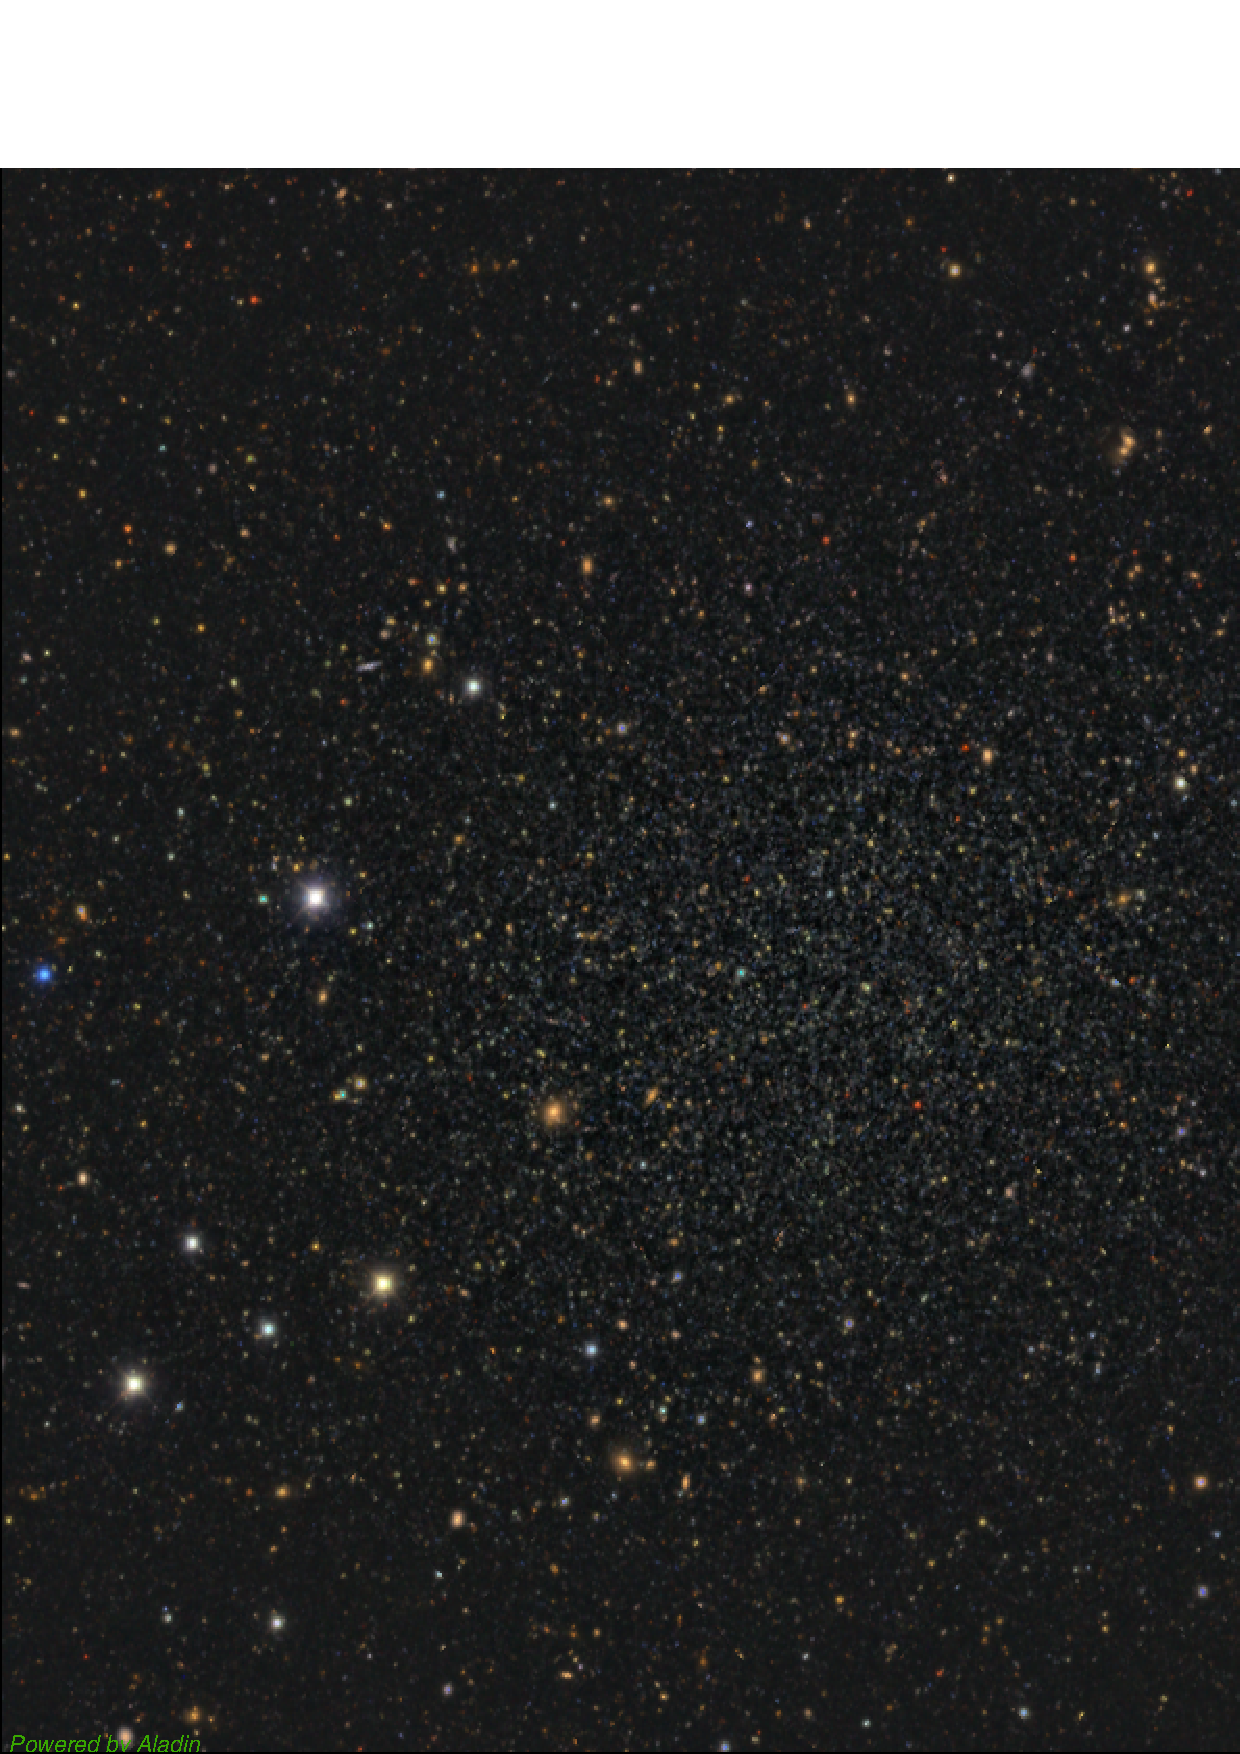
\includegraphics[width=5.41667in,height=5.41667in]{/Users/daniel/thesis/figures/scl_des_dr2.png}
\caption[Picture of Sculptor]{Image of the Sculptor dwarf spheroidal
galaxy from Dark Energy Survey Data Release 2 {[}\citet{abbott+2021};
image created with HiPS2FITS{]}. Sculptor appears as a fairly prominent,
extended over density of predominantly faint, red stars. 0.5 degree
field of view centred on Sculptor. \textbf{TODO: combine with UMi, maybe
add LMC and Fornax?}}\label{fig:scl_image}
\end{figure}

\begin{figure}
\centering
\includegraphics[width=5.41667in,height=5.41667in]{figures/umi_DSS2_0.75deg.png}
\caption[Picture of Ursa Minor]{Image of Ursa Minor dwarf galaxy from
the Digitized Sky Survey 2 (0.75 deg field of view tangent plane). UMi
appears as a diagonal/elliptical haze of faint, reddish stars from the
top left to the bottom right. Even as classical dwarf, Ursa minor is
fairly diffuse and does not stand obviously out from the
background.}\label{fig:umi_image}
\end{figure}

\begin{figure}
\centering
\pandocbounded{\includegraphics[keepaspectratio]{figures/mw_satellites_ongaia.pdf}}
\caption[Dwarf galaxies sky position]{The location of MW dwarf galaxies
on the sky. Dwarf galaxies are taken as confirmed dwarfs with MW or LMC
hosts from the \citet{pace2024} catalogue (version 1.0.3. We label all
classical dwarfs and the Magellanic clouds, changing symbols based on
the relevance to this work (classical dwarfs, Magellanic clouds REF, and
the systems in question or comparison). \textbf{TODO: use
abbreviations}}
\end{figure}

\subsection{Cosmological context}\label{cosmological-context}

\begin{figure}
\centering
\includegraphics[width=1\linewidth,height=\textheight,keepaspectratio]{figures/power_spectrum.png}
\caption[Cosmological Power Spectrum]{The matter power spectrum under
different assumptions for dark matter. Dwarf galaxies occupy the middle
and low end of the blue region (10\^{}10 - 10\^{}8 solar masses),
enabling a unique window into properties of dark matter on small scales.
The smaller scales we can understand dark matter, the better we are able
to test different models of dark matter. figure 1 from
\citet{bechtol+2022}.}\label{fig:cosmological_power_spectrum}
\end{figure}

Figure: Density profiles of comological simulated halos, matching
approximantly the NFW formula.

\begin{figure}
\centering
\pandocbounded{\includegraphics[keepaspectratio]{figures/scl_umi_vs_penarrubia.pdf}}
\caption[Idealized simulations match Scl and UMi]{Sculptor and UMi's
profiles are well-matched to \citet{PNM2008}.}\label{fig:toy_profiles}
\end{figure}

\subsection{Theoretical Background}\label{theoretical-background}

\begin{itemize}
\tightlist
\item
  Cosmology foundations

  \begin{itemize}
  \tightlist
  \item
    power spectrum plot
  \end{itemize}
\item
  NFW plot (density or energy), maybe borrow from paper?

  \begin{itemize}
  \tightlist
  \item
    Explain origin of NFW
  \end{itemize}
\item
  Dwarf galaxy formation, halos
\end{itemize}

N-body DM simulations

\begin{itemize}
\tightlist
\item
  Collisionless Boltzmann equation and meaning of such simulations
\item
  Assumptions \& context \& past work
\item
  Evolution under tidal field
\end{itemize}

To motivate why a tidal interaction may give rise to the observed
density profiles, we create a toy simulation following \citet{PNM2008}.

\begin{itemize}
\item
  NFW initial conditions (sculptor like, vcm, rcm)
\item
  Evolved in x-y plane using \citet{EP2020} potential for
  \textasciitilde{} 5Gyr with pericentre of 15 kpc and apocentre of 100
  kpc.
\item
  Exponential initial stellar profile.
\end{itemize}

As a dark matter halo is perturbed on a pericentric passage with the
milky way,

\begin{itemize}
\tightlist
\item
  Tidal stress heats halo slightly
\item
  Mass loss, particularly of loosely bound particles
\end{itemize}

The stellar component tracers will similarly follow the behaviour of the
dark matter.

An emperical estimate of where the simulation's stars are becoming
unbound is, as stated in \citet{PNM2008}, the break radius
\begin{equation}
R_b = C\,\sigma_{v}\,\Delta t
\end{equation} where \(\sigma_v\) is the present line of sight velocity
dispersion , \(\delta t\) is the time since pericentre, and
\(C \approx 0.55\) is a fit. The idea motivating this equation is stars
in the inner regions will have dynamically equilibriated to the new
potential (phase mixed), however the outer regions are no longer in
steady state, so we have to wait until the crossing time reaches them as
well.

As illustrated in fig.~\ref{fig:toy_profiles}, the density profile
initially stars off exponential. At increasing times since the first
pericentric passage, the break radius, appearing as an apparent
separation between the slopes of the inner and outer profile, increases.

\subsection{Introduction to Dark Matter
simulations}\label{introduction-to-dark-matter-simulations}

In this section, we will cover

\begin{itemize}
\tightlist
\item
  How are dark matter simulations conducted
\item
  Interpretations and uncertainties
\item
  Methods
\end{itemize}

\begin{figure}
\centering
\pandocbounded{\includegraphics[keepaspectratio]{/Users/daniel/thesis/figures/idealized_break_radius.png}}
\caption[Break radius validation]{The break radius of the simulations is
set by the time since pericentre.}\label{fig:idealized_break_radius}
\end{figure}

From this argument, we note that the following properties must be
approximately true for tides to occur:

\begin{itemize}
\tightlist
\item
  Close enough pericentre. The other break radius \(r_J\) implies that
  if the host density is 3x the satellite, stars will be lost
\item
  Corresponding time since last pericentre: If the time since last
  pericentre is not \(\sim\) consistent with an observed break in the
  density profile, then tides
\item
  Halo evolution. As found in \citet{EN2021}, galaxies evolve along well
  defined tidal tracks (assuming spherical, isotropic, NFW halo, which
  may not be true, see \ldots). These tracks tend to ``puff up'' the
  stellar component while also removing dark matter mass, leaving a
  smaller, compacter DM halo with a more extended stellar component.

  \begin{itemize}
  \tightlist
  \item
    This information is mostly related to the statistical initial
    distribution of satellites from cosmology {[}ludlow+2016;
    \citet{fattahi+2018}{]}
  \end{itemize}
\end{itemize}

\subsection{Potentials}\label{potentials}

From the \citet{nfw1996} paper, eqns. 3 \& 4 \begin{equation}
\frac{\rho}{\rho_c} = \frac{\delta_c}{(r/r_s)(1+r/r_s)^2}
\end{equation} where \begin{equation}
\delta_c = \frac{200}{3}\frac{c^3}{[\ln(1+c)-c/(1+c)]}
\end{equation} \(c\) is concentration parameter, \(\rho_c\) is the
critical density of the universe, and \(r_s\) is the characteristic
scale length of the halo.

The NFW halo is sometimes described by \(M_{200}\). \(r_{200}\) is the
radius at which the mean density of the halo interior to \(r_{200}\) is
200 times the critical density of the universe, and \(M_{200}\) is the
mass contained inside \(r_{200}\). As equations: \begin{equation}
\rho_{200} = 200\rho_{c} = \frac{M_{200}}{(4\pi/3) r_{200}^3}
\end{equation}

\begin{equation}
r_{200} = \sqrt[3]{\frac{1}{200}\frac{3M_{200}}{4\pi \rho_{\rm c
}}}
\end{equation}

\begin{equation}
M_{200} = \frac{4\pi}{3} r_{200}^3\ \rho_{200}
\end{equation}

\(M_{200}\) is also sometimes called the virial mass of the halo.
\(r_{200}\) is directly related to \(r_s\) by \begin{equation}
r_{200} = c\,r_s
\end{equation}

Another useful definition is \begin{equation}
A(x) \equiv \log (1+x) - \frac{x}{1+x}.
\end{equation}

We will also define a dimensionless radius \begin{equation}
x \equiv r/r_s.
\end{equation}

A simple substitution to the definition gives

\begin{equation}
\rho(x) =  \frac{\rho_s/3}{x\ (1+x)^2}
\end{equation} where \begin{equation}
\rho_s = \frac{c^3}{A(c)} \rho_{200}
\end{equation} and \(A(c)\) is as above. The characteristic density can
also be written in terms of scale mass, \(M_s = M_{200}/{A(c)}\) (see
below), giving \begin{equation}
\rho_s = \frac{c^3}{A(c)} \frac{M_{200}}{(4\pi/3)\ r_{200}^3}  = \frac{3M_s}{4\pi\, {r_s}^3}
\end{equation} Note that the NFW density profile is the same as an
alpha-beta-gamma profile where \(\alpha=\gamma=1\) and \(\beta =3\).

\subsubsection{Circular velocity}\label{circular-velocity}

The circular velocity in terms of
\(v_{200} = \sqrt{G M_{200} / R_{200}}\) is \begin{equation}
\left(v_{\rm circ}/v_{200}\right)^2 = \frac{A(x)/x}{A(c)/c},
\end{equation}

or in terms of \(M_s\) and \(r_s\), \begin{equation}
v_{\rm circ}^2 = \frac{G M(r)}{r} = \frac{G M_s A(r/r_s)}{r}.
\end{equation} Another parameterization of the NFW profile is in terms
of the maximum circular velocity \(v_{\rm circ}^{\rm max}\) and the
radius at which it is reached \(r_{\rm circ}^{\rm max}\). Given the
scale radius, \begin{equation}
r_{\rm circ}^{\rm max} = \alpha\ r_s
\end{equation}

where \(\alpha\approx2.16258\), and \(v_{\rm circ}^{\rm max}\) can be
found from either of the equations above.
